\documentclass[
 reprint,
 amsmath,amssymb,
 aps,
]{revtex4-1}


\usepackage{graphicx}% Include figure files
\usepackage{dcolumn}% Align table columns on decimal point
\usepackage{bm}% bold math
\usepackage{glossaries}     % Enable the \newacronym and \gls commands to reference terms
\usepackage{commath}        % We have this here to use the \abs{} equation function
\usepackage{amssymb}
% \usepackage{svg}
\usepackage{mathtools}
\usepackage{booktabs}
\usepackage{array}
\usepackage{makecell}
\usepackage{todonotes}
% \renewcommand\theadalign{bc}
\renewcommand\theadfont{\bfseries}
\usepackage{multirow}
\newcommand{\ang}{\mbox{\normalfont\AA}}
\newacronym{DFT}{DFT}{Density Functional Theory}
\newacronym{onlineal}{Online-AL}{Online Active Learning}
\newacronym{offlineal}{Offline-AL}{Offline Active Learning}

\newacronym{mlp}{MLP}{Machine Learning Potential}
\newacronym{QE}{QE}{Quantum Espresso}
\newacronym{VASP}{VASP}{Vienna Ab initio Simulation Package}

\begin{document}

\title{Supporting Information}

\author{Muhammed Shuaibi, Saurabh Sivakumar, Rui Qi Chen}
%  \email{mshuaibi@andrew.cmu.edu}
\author{Zachary W. Ulissi}%
 \email{zulissi@andrew.cmu.edu}
\affiliation{%
Department of Chemical Engineering, Carnegie Mellon University, Pittsburgh, PA 15213, United States
}%

\date{\today}
            
             
\section{Supplementary Information}
\renewcommand{\theequation}{S.\arabic{equation}}
\renewcommand\thefigure{S.\arabic{figure}}
\setcounter{figure}{0}  
\setcounter{equation}{0}
\subsection{High-temperature MD}
In a similar manner to Figure 4 of the main text, we demonstrate our framework's ability to successfully converge to an accurate high-temp MD despite the highly perturbed sampled configurations. This same experiment was unsuccessful without the inclusion of the more potential prior we have introduced in this work. Beginning with a dataset containing a single structure, we run the proposed framework over a 2ps MD simulation of CO on Cu(100) in a 800K NVT ensemble. We illustrate our results in Figure \ref{fig:almd_800k}, with good agreement as early as the 3rd iteration - suggesting that the sampled highly-perturbed structures aid in reaching a converged simulation in much fewer iterations.

\begin{figure*}[ht!]
    \centering
    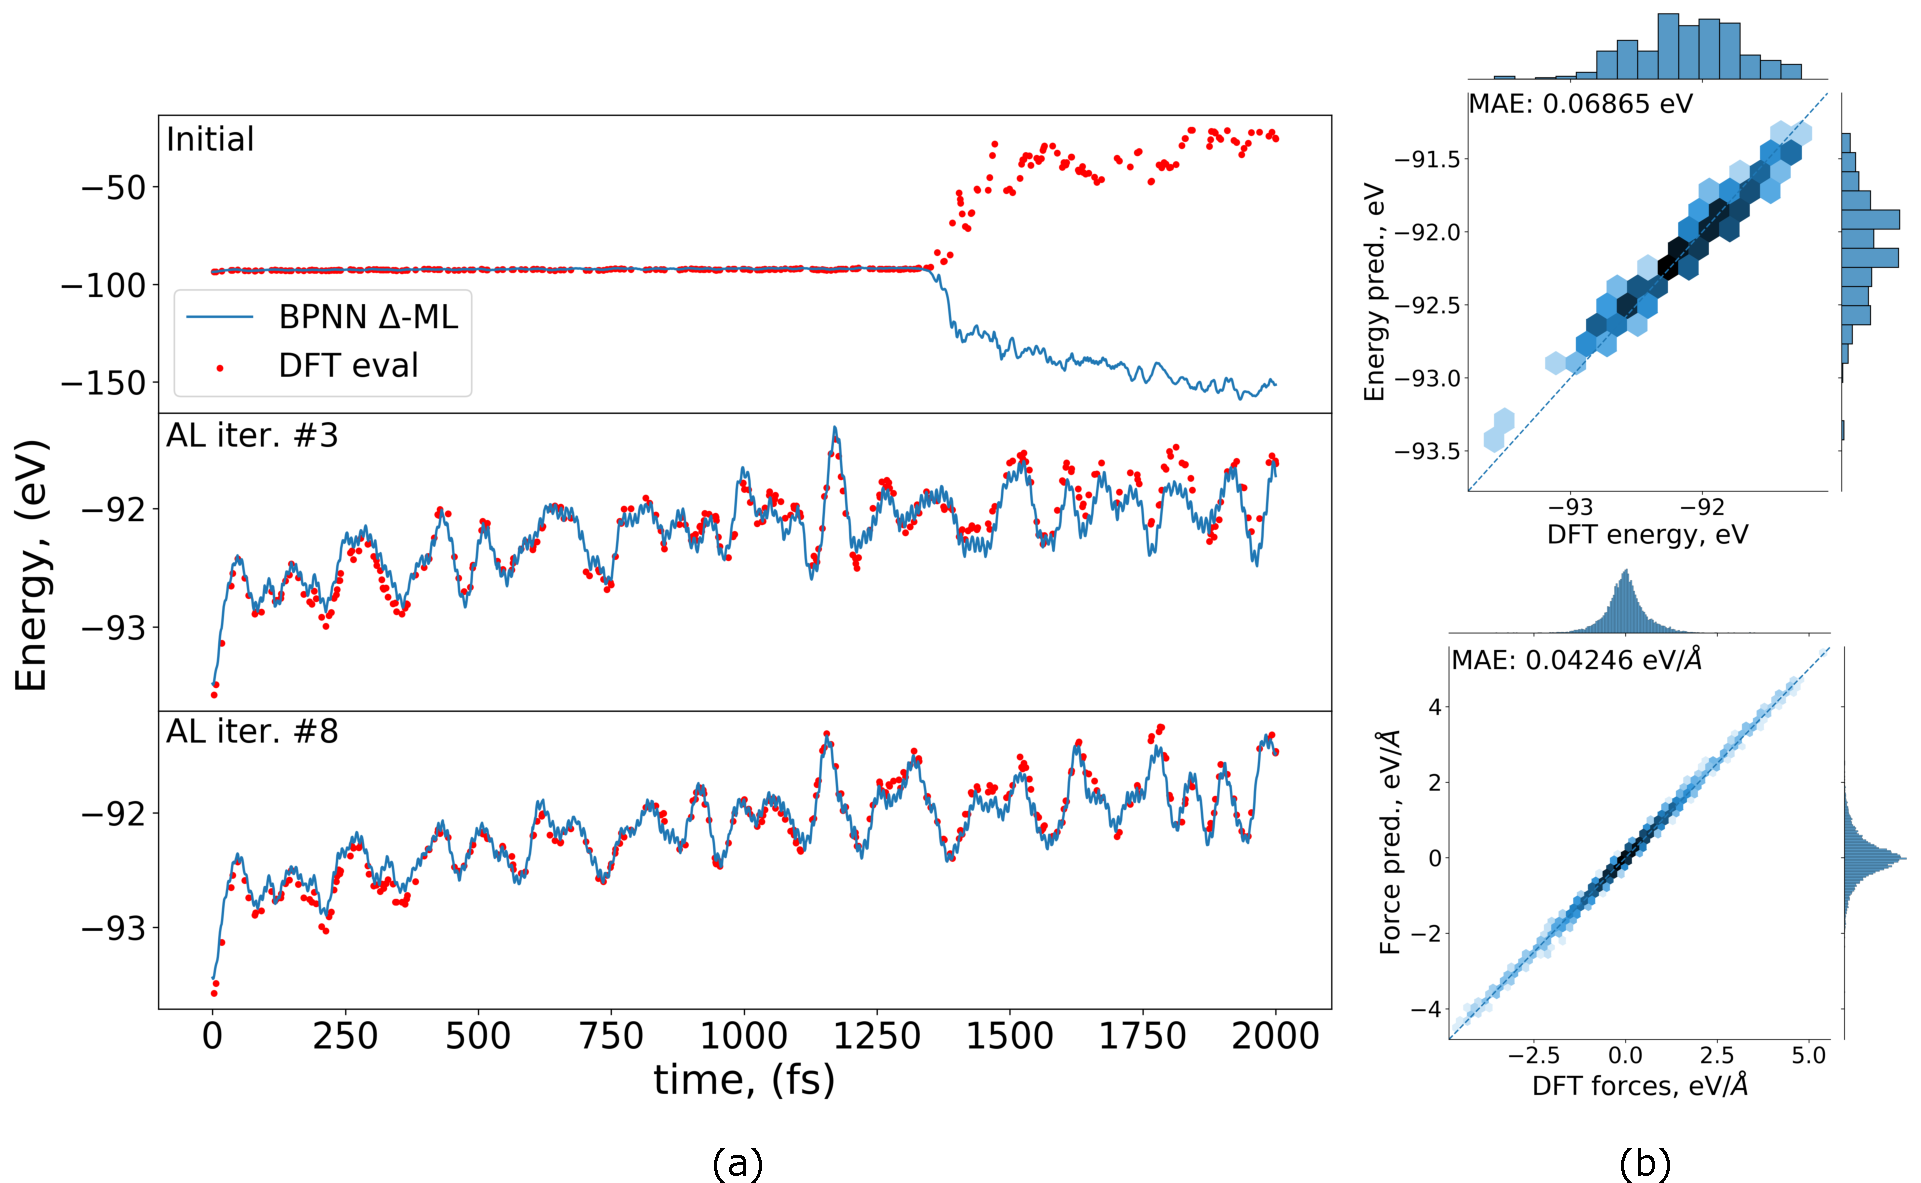
\includegraphics[width=\textwidth]{figures/figure_s1.pdf}
    \caption{ \gls{offlineal} demonstration to a 2ps MD simulation of CO on Cu(100) at 800K\textbf{(a)} Evolution of the MD trajectory over several iterations of the active learning framework. We verify the effectiveness of our framework by randomly sampling configurations and comparing DFT evaluated energy and forces with that of our model's predictions. \textbf{(b)} Parity plots associated with the DFT evaluated configurations and our model's predictions on the 8th iteration, demonstrating good agreement. Shading was scaled logarithmically with darker shading corresponding to a higher density of points. 
    }
    \label{fig:almd_800k}
\end{figure*}

\subsection{Interactive examples}
Several interactive Google Colab notebooks have been prepared to allow readers to conveniently explore the proposed methods. Accelerated structural relaxations and transition state calculations can be found at Ref \cite{examples}. Random query strategies are used to demonstrate the effectiveness of even the simplest of strategies. We encourage users to explore query and termination strategies that best suites their application of choice. DFT calculations are performed directly in the notebook examples via a GPU-enabled Quantum Espresso package.

\subsection{Morse parameters fitting}
The Morse potential was selected for our primarily bonded, catalytic systems. Parameters of the Morse potential, $D_e$, $r_e$, and $a$, corresponding to well depth, equilibrium distance, and well width were computed in the following manner for a given element, X:
\begin{enumerate}
    \item Lone atomic energies, $E_X$, obtained through singlepoint DFT calculations;
    \item Diatomic atoms relaxed to obtain a relaxed state energy, $E_{X_2}$, and equilibrium distance, $r_e$.
    \item Well depth, $D_e$, is calculated as follows:
    \begin{equation}
        D_e = -(E_{X_2} - 2 * E_X)
    \end{equation}
    \item Diatomic bond stretched and corresponding DFT points fit to Morse potential functional form (\ref{morse}) to obtain $a$ Figure (\ref{fig:morsefit}).
    \begin{equation}\label{morse}
    E_{morse} = D_e(e^{-2a(r-r_e)} - 2e^{-a(r-r_e)})
    \end{equation}
\end{enumerate}
 
To make use of the Morse potential for multi-element systems, linear mixing rules are utilized to compute element pair parameters. Adapted from Yang, et al.\cite{Yang2018} the Morse potential is rewritten and parameter combinations applied accordingly (\ref{newmorse}-\ref{mix3})
\begin{equation}\label{newmorse}
    E_{morse} = D_e(\exp[{-\frac{2C}{\sigma}(r-r_e)}] - 2\exp[{-\frac{C}{\sigma}(r-r_e)})]
\end{equation}
\begin{flalign}
    D_{AB} &= \sqrt{D_AD_B} \label{mix1}\\ 
    r_{e, AB} &= \frac{r_{e, A} + r_{e, B}}{2} \label{mix2}\\
    \sigma_{AB} &= \frac{\sigma_{A} + \sigma_{B}}{2} \label{mix3}
\end{flalign}
Where $C = \ln{2}/(r_e - \sigma)$ and $\sigma$ corresponds to $E_{morse}(\sigma) = 0$. Although more sophisticate combination rules exist \cite{Yang2018}, the accuracy of our Morse potential is not crucial for the success of our framework as it is meant to provide some guidance to the model.\\

\subsection{Convergence}

The convergence of the \gls{offlineal} loop can be accelerated through the use of a learning rate scheduler. Figure \ref{fig:scheduler} compares the learning curves of AL frameworks with and without a learning rate scheduler, ceteris paribus. We demonstrate that a cosine annealing scheduler with warm restarts \cite{loshchilov2016sgdr} was able to assist the convergence by smoothing out the learning curve and requiring fewer training images to reach a similar level or error.

\begin{figure*}[!th]
    \centering
    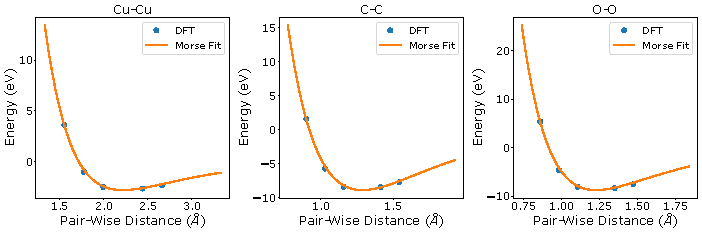
\includegraphics[width=\textwidth]{figures/figure_s2.pdf}
    \caption{Morse parameters are obtained by fitting DFT points near the equilibrium distance to equation \ref{morse}. Sample fittings are illustrated for copper, carbon, and oxygen.} 
    \label{fig:morsefit}
\end{figure*}  

\begin{figure*}
    \centering
    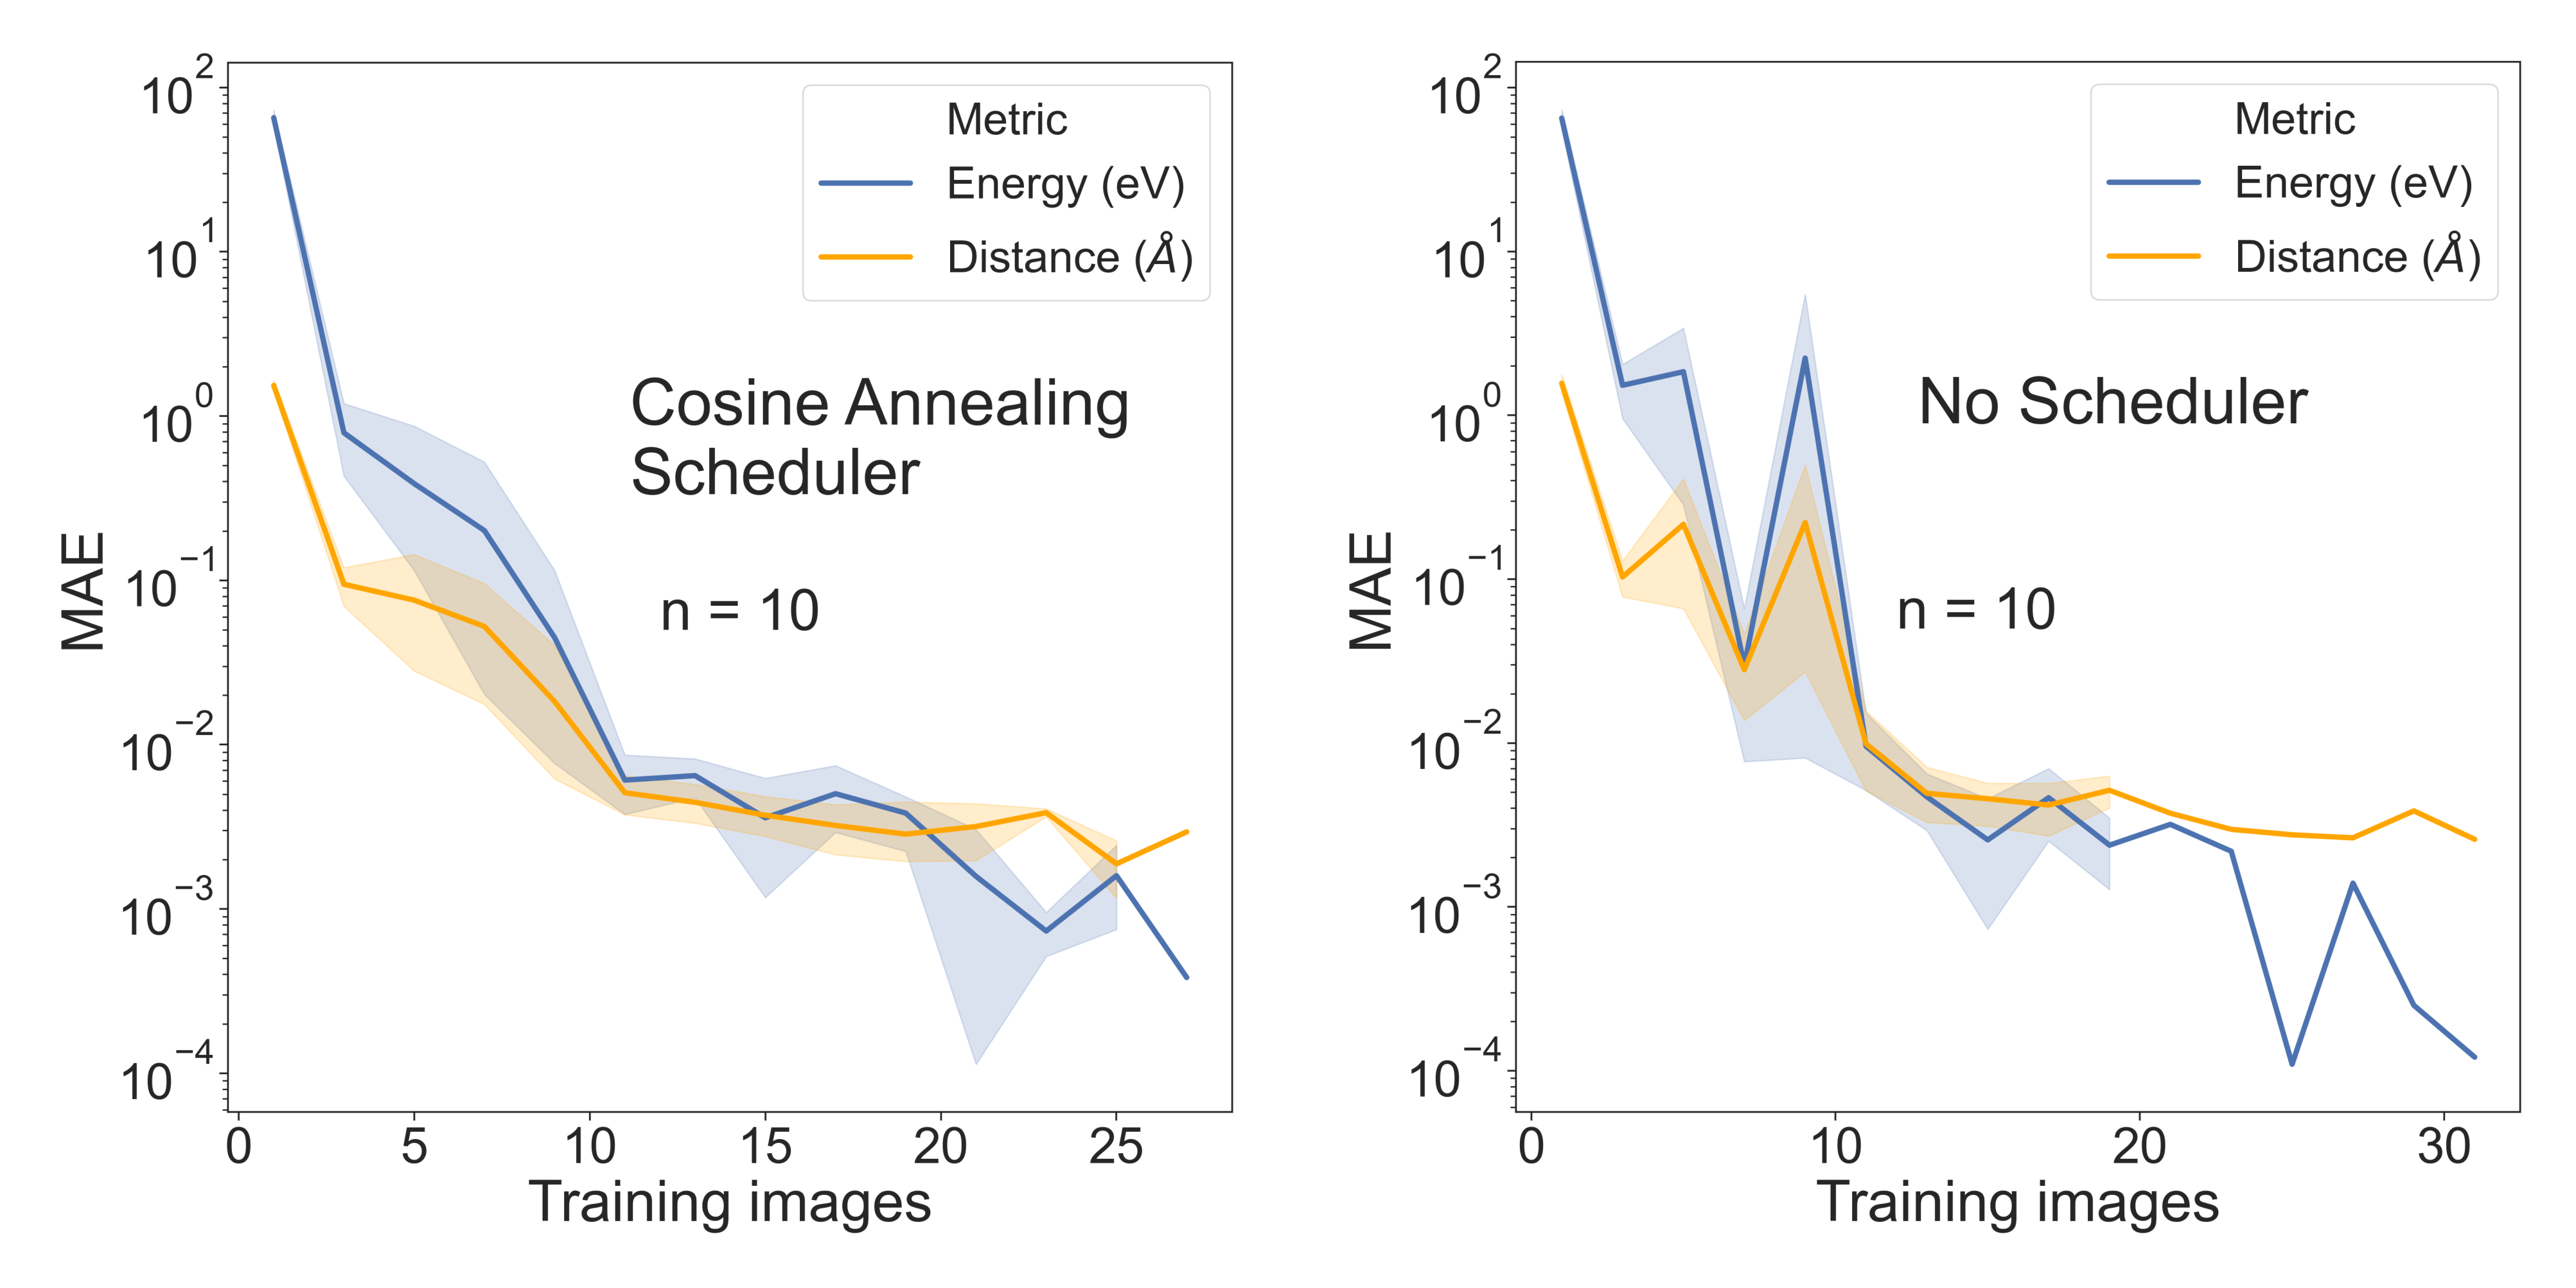
\includegraphics[width=\textwidth]{figures/figure_s3.pdf}
    \caption{Offline-AL convergence of our BPNN $\Delta$-ML is compared with and without a learning rate scheduler. The use of a scheduler, particularly with small data, enables our framework to converge more reliably to the local minima.}
    \label{fig:scheduler}
\end{figure*}
\bibliography{main_paper}% Produces the bibliography via BibTeX.
\end{document}

